\chapter{Data} \label{data}

\begin{figure}[t]
 \centering
 \begin{tabular}{cc}
 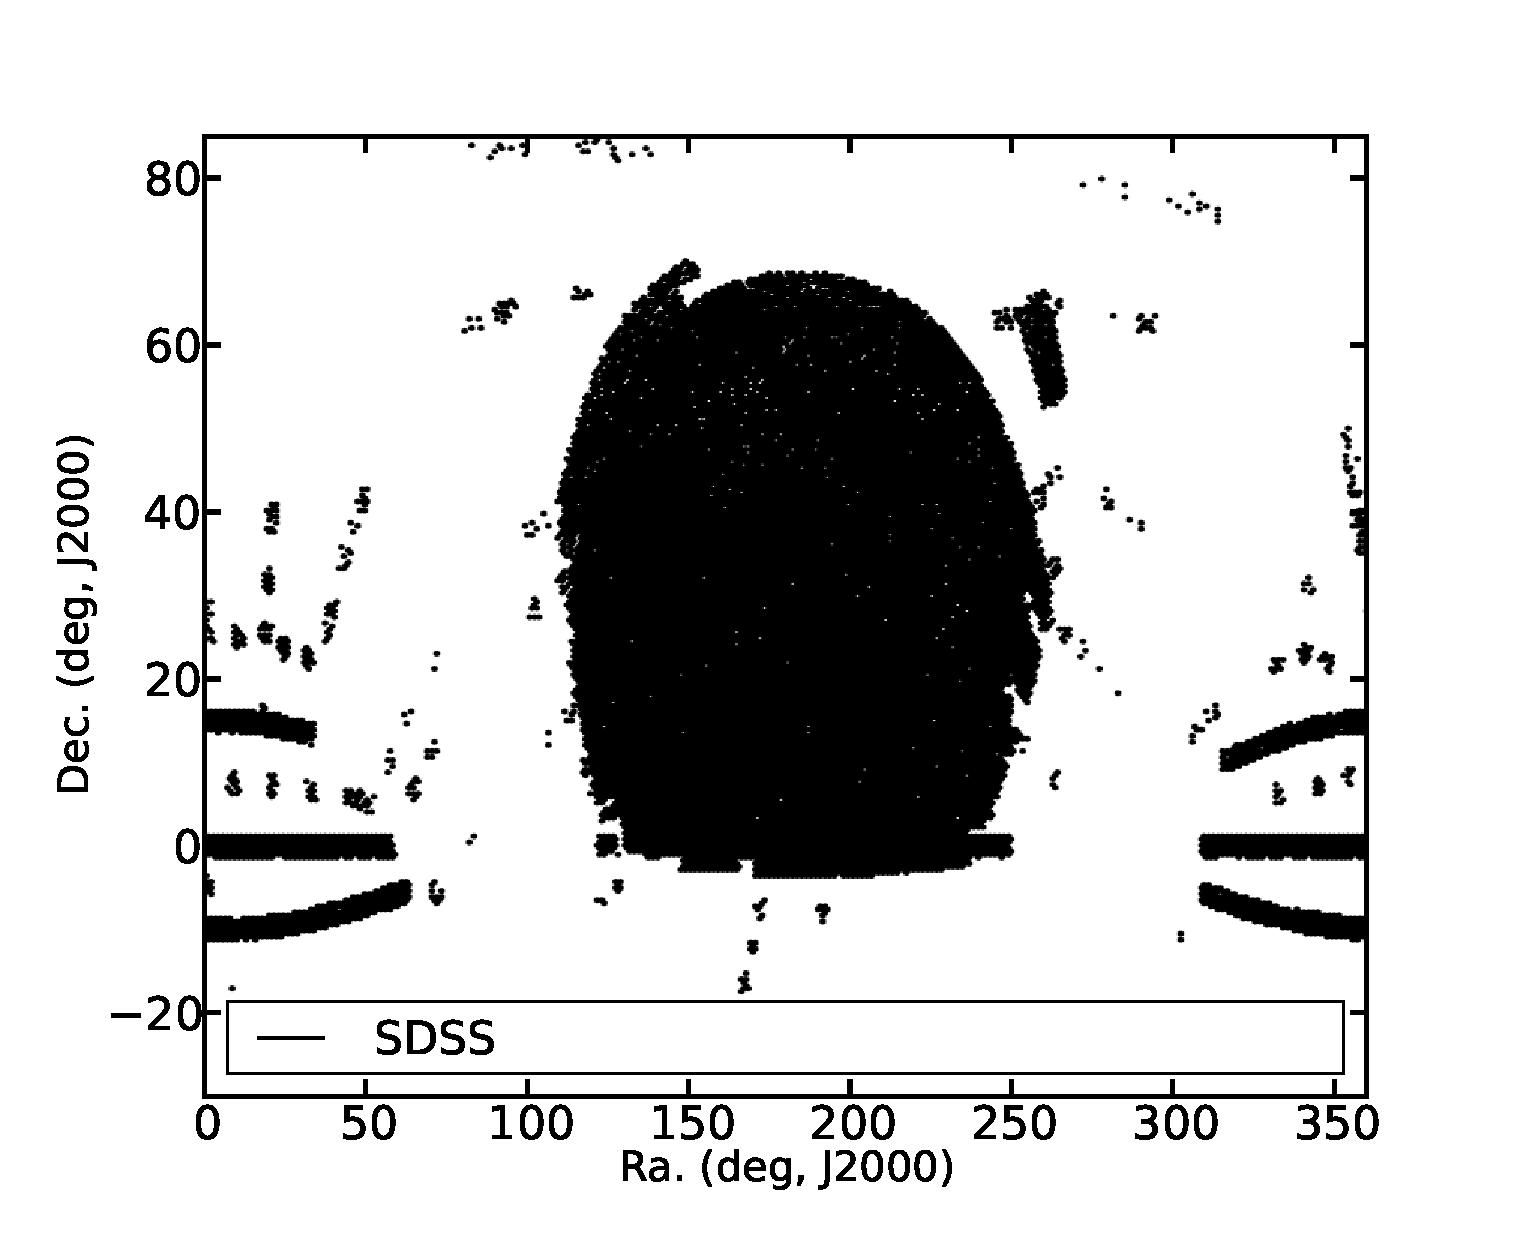
\includegraphics[width=3in]{images/Data/f1a} & 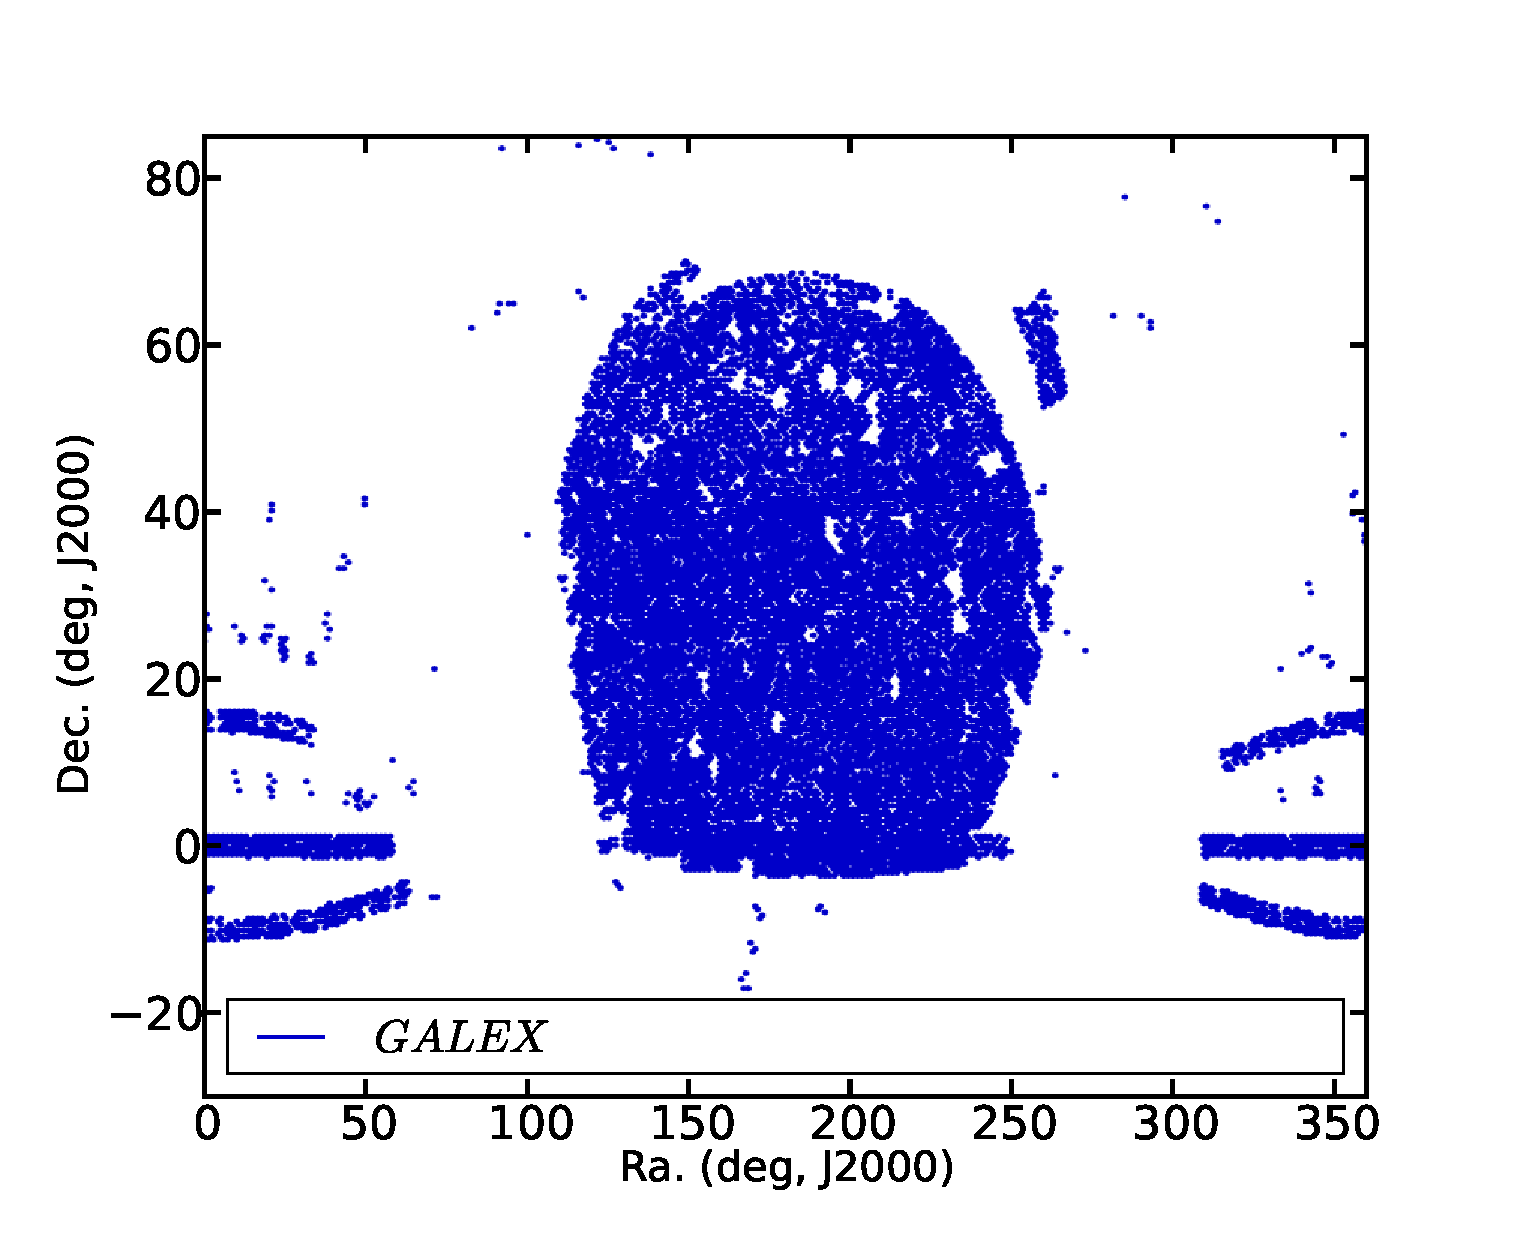
\includegraphics[width=3in]{images/Data/f1b} \\
 (a) SDSS quasar footprint & (b) {\em GALEX} quasar footprint \\
 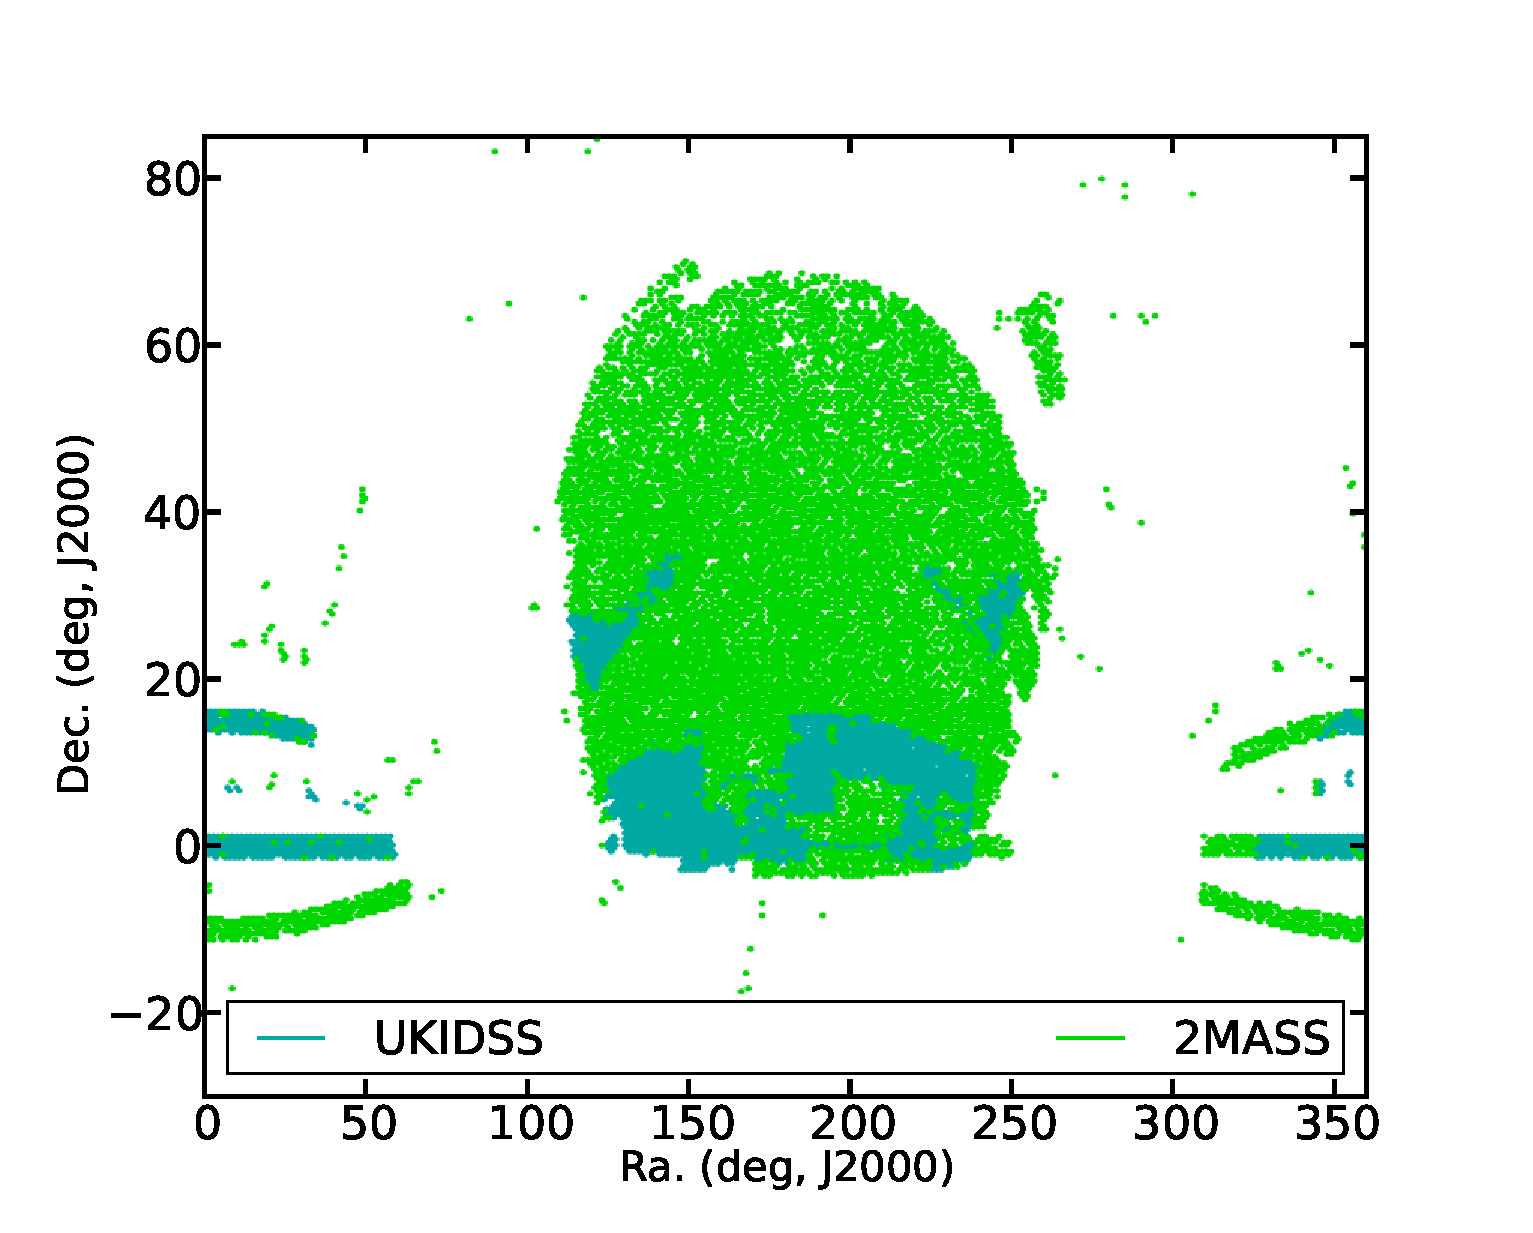
\includegraphics[width=3in]{images/Data/f1c} & 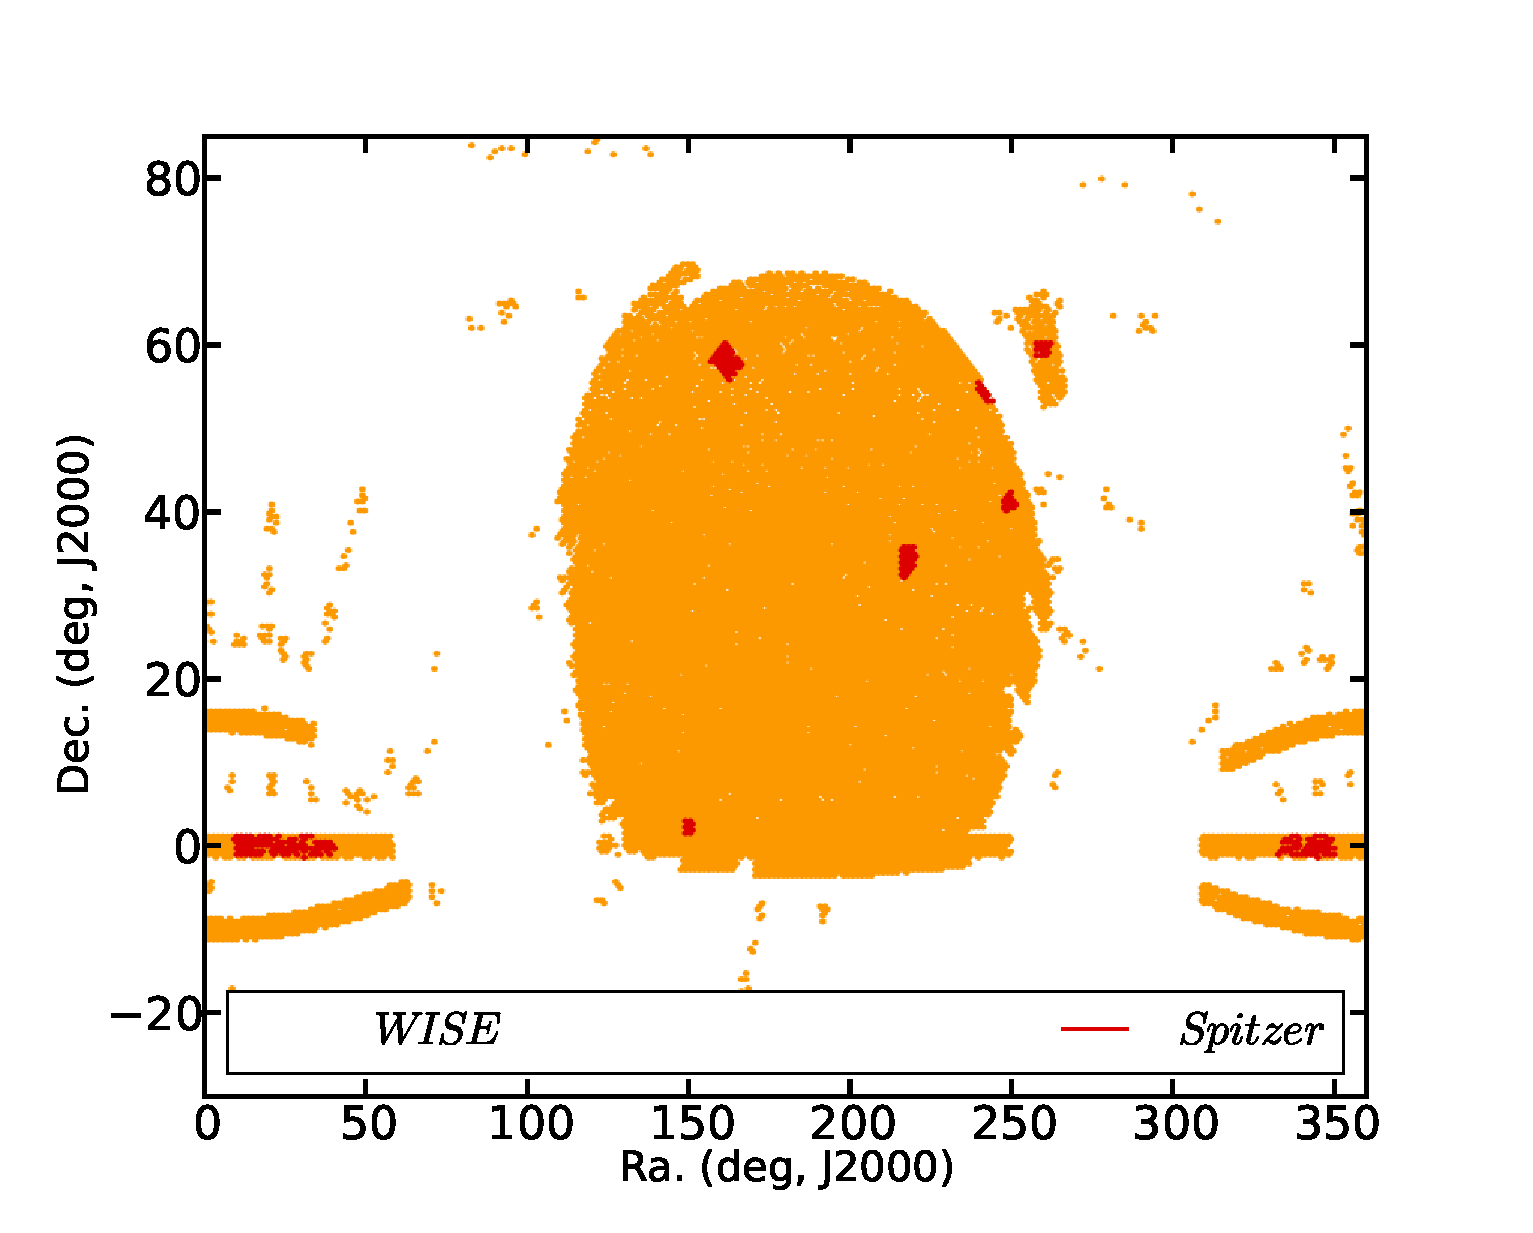
\includegraphics[width=3in]{images/Data/f1d} \\
 (c) Near-IR quasar footprint & (d) Mid-IR quasar footprint
 \end{tabular}
 \caption[Matched survey footprints]{Footprints of the optically selected quasars in the matched surveys.  Coverage of {\em GALEX} (blue), UKIDSS (teal), 2MASS (green), {\em WISE} (orange), and {\em Spitzer} (red) data are limited to the SDSS footprint (black) shown in the top-left panel.}
\label{foot}
\end{figure}

Our sample starts with the SDSS-DR7 quasar catalog by \citet{Schneider:2010}, containing 105,783 spectroscopically confirmed broad-lined quasars.  Each quasar has photometric data in the five SDSS optical bandpasses $ugriz$ \citep{Fukugita:1996}.  
Only quasars that have nonzero flux in all five SDSS bandpasses after correcting for Galactic extinction have been kept in our catalog, bringing the sample size to 103,895.
While the SDSS survey covers a large area of sky, it is limited to relatively bright quasars ($i<19.1$ for $z<3$ and $i<20.2$ for $z>3$).  As such, in addition to these quasars, we included 15,757 lower luminosity, optically-selected quasars taken from the Two Degree Field QSO Redshift survey \citep[2QZ; $b_J<20.85$ for $z<3$;][]{Croom:2004}, the Two Degree Field-SDSS LRG and QSO survey \citep[2SLAQ; $g<21.85$ for $z<3$;][]{Croom:2009}, and the AAT-UKIDSS-SDSS survey (AUS; $i<21.6$ for $0<z<5$; Croom et al., in preparation). 
In the rest frame, we have over 70,000 QSOs with $\log{(\nu [{\rm Hz}])}$ ranging from $\sim$13.7--15.4 ($\lambda\sim$1200\,\AA--6\,$\mu$m) and at least 10,000 QSOs covering the range from $\sim$13.3--15.6 ($\lambda\sim$750\,\AA--15\,$\mu$m).
All SDSS magnitudes have been corrected for Galactic extinction according to \citet{Schlegel:1998} with corrections to the extinction coefficients as given by \citet{Schlafly:2011}. 
 Table~\ref{data_table} presents the IR--UV photometry for the 119,652 quasars in our sample.  
 Signs of dust reddening are seen in 11,468 of these, specifically with a color excess $\Delta(g-i) > 0.3$ \citep{Richards:2003}. 
 In Chapter~\ref{SEDs}, these have been excluded from our analysis, bringing our final sample size to 108,184. However, in Chapter~\ref{Dust}, we explicitly study the dust reddening properties of quasars, so these objects are added back into the sample.
 Figure~\ref{foot} shows the sky coverage of our multi-wavelength data and Figure~\ref{lum_v_z_survey} shows the 2500\,\AA\ luminosity versus redshift distributions for each survey.
Note that, in the so-called SDSS ``Stripe 82'' region \citep{Annis:2011} along the Northern Equatorial Stripe, the SDSS imaging data reaches roughly 2 mag deeper than the main survey as a result of co-adding many epochs of data.  

\begin{figure}[t]
\centering
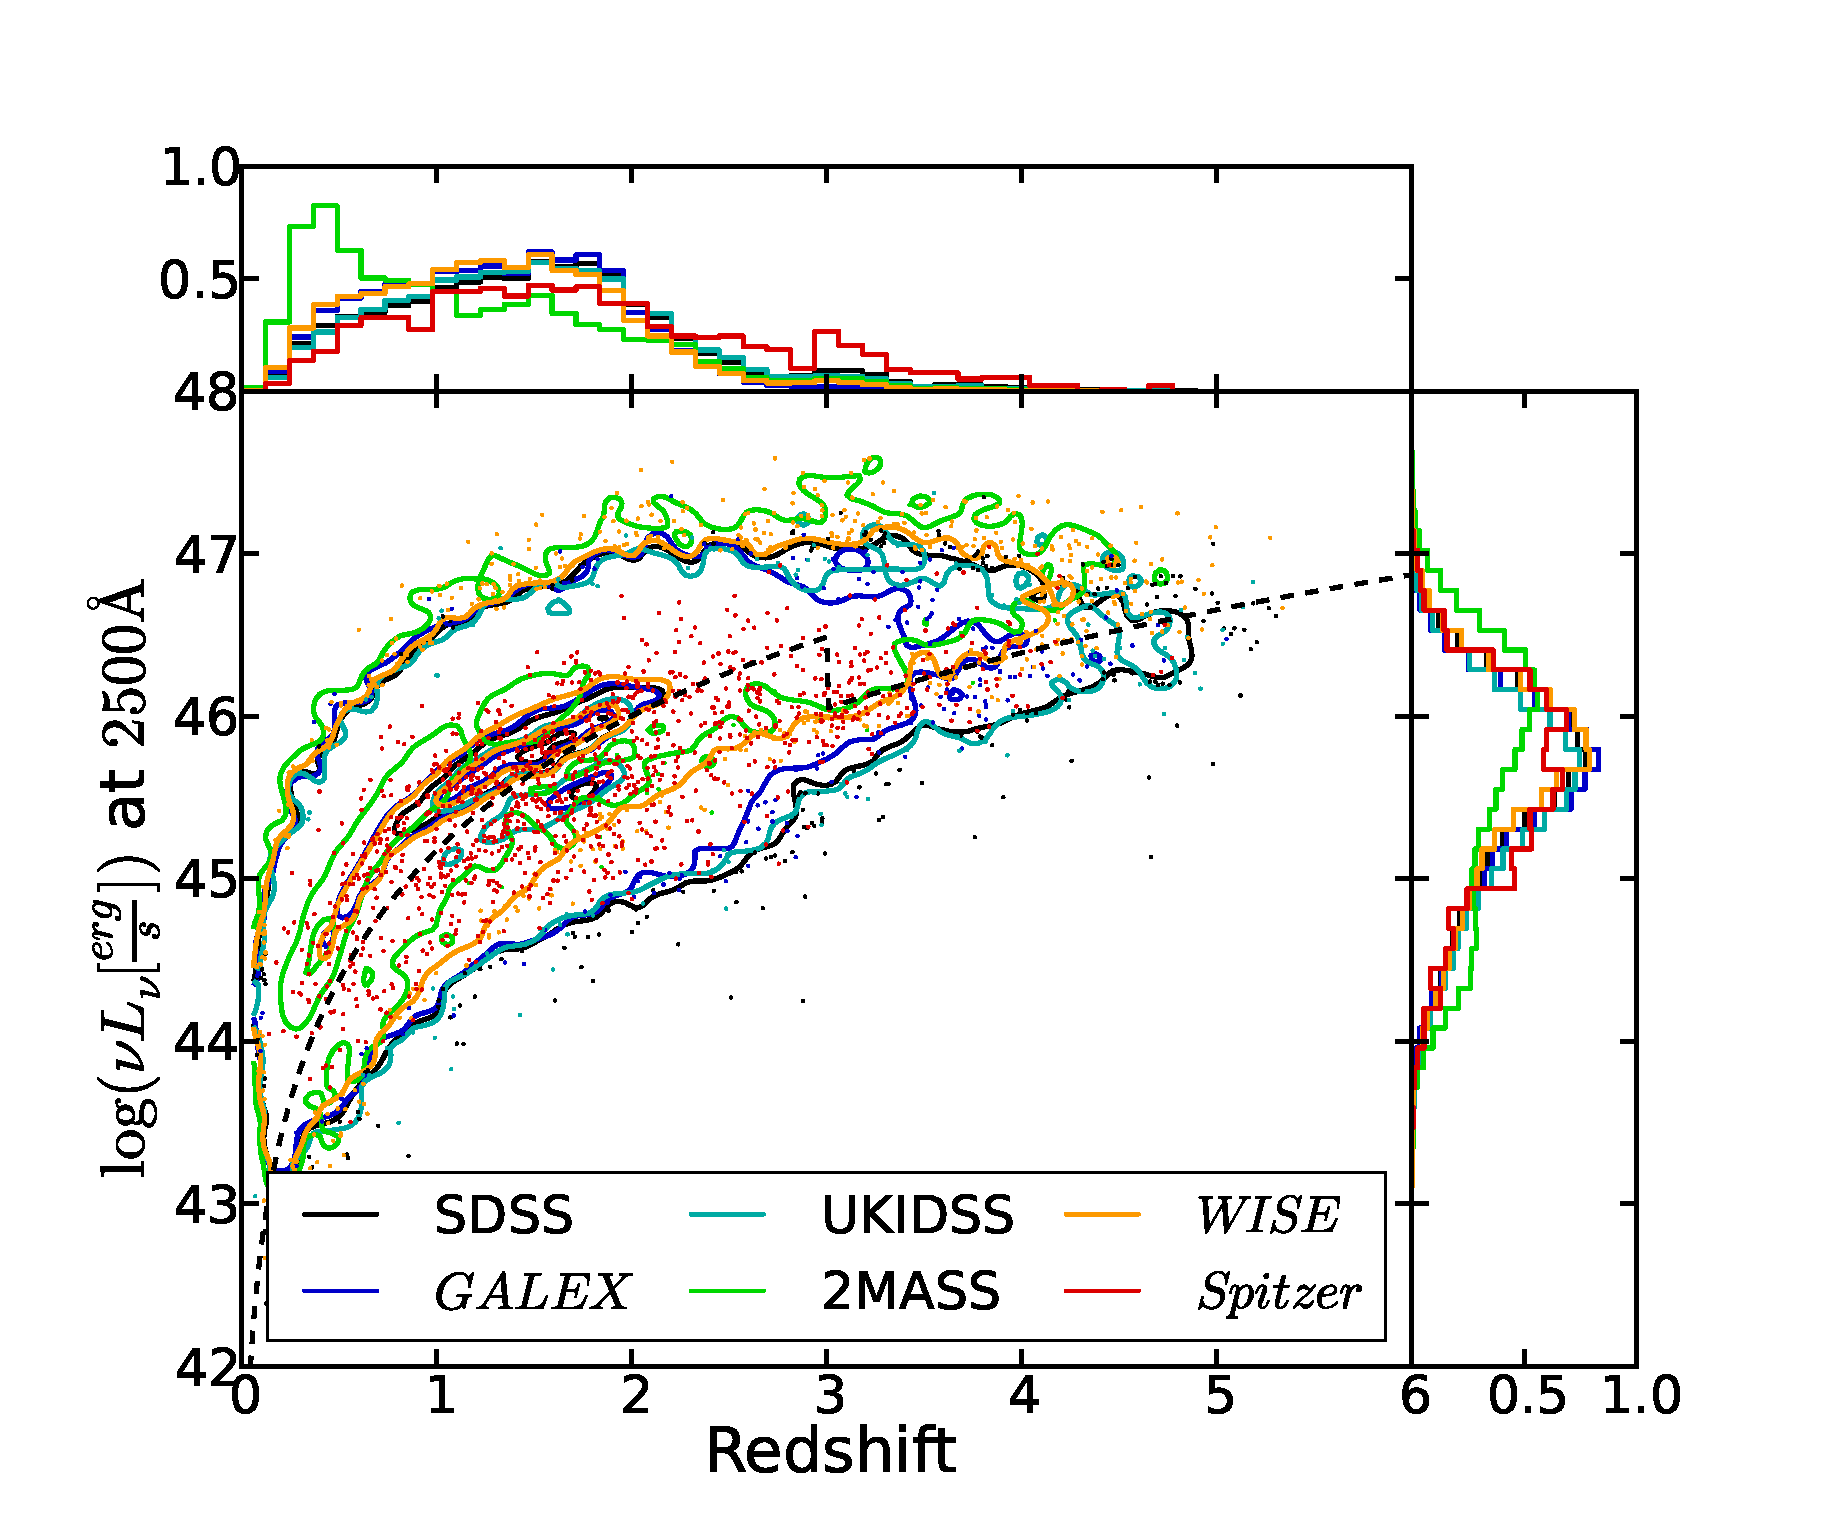
\includegraphics[width=5in]{images/Data/f2}
\caption[Luminosity vs. redshift]{Contour-scatter plot showing the 2500\,\AA\ luminosity vs. redshift for each quasar color coded by survey. The contours indicate the linear density of scatter points on the plot with level drawn at 0.005, 0.5, and 0.95 of the normalized distributions.  The histograms are normalized by the total number of quasars in each survey:  119,652 in SDSS, 42,043 in {\em GALEX}, 35,749 in UKIDSS, 23,088 in 2MASS, 85,358 in {\em WISE}, and 1196 in {\em Spitzer}.  The black dashed line represents the flux limit of the main SDSS survey before extending the sample to lower luminosities.}
\label{lum_v_z_survey}
\end{figure}

\setlength{\tabcolsep}{4pt}

\begin{deluxetable}{ll}
\tabletypesize{\footnotesize}
\tablewidth{0pt}

\tablecaption{Quasar Catalog Format \label{data_table}}
\tablehead{\colhead{Column} & \colhead{Description}}
\startdata
1   &   Previously published name\\
2   &   Right ascension in decimal degrees (J2000)\\
3   &   Declination in decimal degrees (J2000)\\
4   &   Redshift       \\
5   &    BEST SDSS {\em u} band PSF magnitude\\
6   &    Error in {\em u} magnitude\\
7   &    BEST SDSS {\em g} band PSF magnitude\\
8   &    Error in {\em g} magnitude  \\
9   &    BEST SDSS {\em r} band PSF magnitude\\
10  &    Error in {\em r} magnitude  \\
\enddata
\tablecomments{This table is available in its entirety in a machine-readable form in the journal publication \citet{Krawczyk:2013}.
A portion is shown here for guidance regarding its form and content.}
\end{deluxetable}

\section{Near-Infrared}

Near-IR data in the {\em JHK} bandpasses are taken from the Two Micron All Sky Survey \citep[2MASS;][]{Skrutskie:2006}.  These include values that were matched to the 2MASS All-Sky and ``6$\times$'' point source catalogs using a matching radius of $2''$ with the 6$\times$ deeper catalog taking priority.  In addition to these data, we include 2$\sigma$ extractions (i.e., ``forced photometry'') at the positions of known SDSS quasars.  These objects have sufficiently accurate optical positions that it is possible to perform aperture photometry at their expected locations in the near-IR imaging, despite being non-detections in 2MASS.  These 2$\sigma$ ``detections'' were cataloged by \citet{Schneider:2010}; we include those objects with a signal-to-noise ratio (S/N) greater than 2.

To supplement the 2MASS data, we have matched our catalog to the UKIRT (United Kingdom Infrared Telescope) Infrared Deep Sky Survey \citep[UKIDSS; ][]{Lawrence:2007}. UKIDSS uses the $YJHK$ filter system \citep{Hewett:2006}; see also \citet{Peth:2011}.  
In order to generate our combined optical and near-IR data sets, we begin by source matching samples of SDSS data with the UKIDSS LAS catalog using the Cross-ID form located on the Web site of the WFCAM Science Archive (WSA)\footnote{\url{http://surveys.roe.ac.uk:8080/wsa/crossID\_form.jsp}}. In particular, we match against the UKIDSS DR5 LAS source table which contains the individual detections for a given object from each bandpass merged into a single entry.
We use a matching radius of 0.\hspace{-.2em}$''$7 and the nearest neighbor pairing option, accepting only the nearest object with a detection in at least one band as an acceptable match.

Since UKIDSS is deeper than 2MASS, when a quasar has data in both surveys, we only use the UKIDSS data. Between UKIDSS and 2MASS, 77,864 of our sample quasars have data in the near-IR: 35,749 from UKIDSS data and 41,434 from 2MASS, including both $5\sigma$ detections and forced photometry. Figure \ref{2mass_v_ukidss} shows the difference between the UKIDSS and 2MASS magnitudes versus the UKIDSS magnitudes for the 12,130 quasars the two surveys have in common.  We have split each figure into three distinct groups: quasars taken from the 2MASS $5\sigma$ catalog, quasars with $2\sigma$ 2MASS extraction values in more than one filter, and quasars with $2\sigma$ 2MASS extractions in only one filter.  As the quasars in the third group have much larger scatter (up to 2.5 mag) that can result in a misestimation of the quasar's luminosity by up to one order of magnitude,
we have removed all quasars that fall into this group.  This process leaves 23,088 objects in our 2MASS sample and brings our total number of QSOs with near-IR data to 58,837. 
In Table \ref{data_table} all 2MASS and UKIDSS fluxes have been converted to the AB magnitudes using \citet{Hewett:2006} conversions between AB and Vega magnitudes for the UKIDSS system.

\begin{figure*}[h]
 \centering
 \begin{tabular}{cc}
 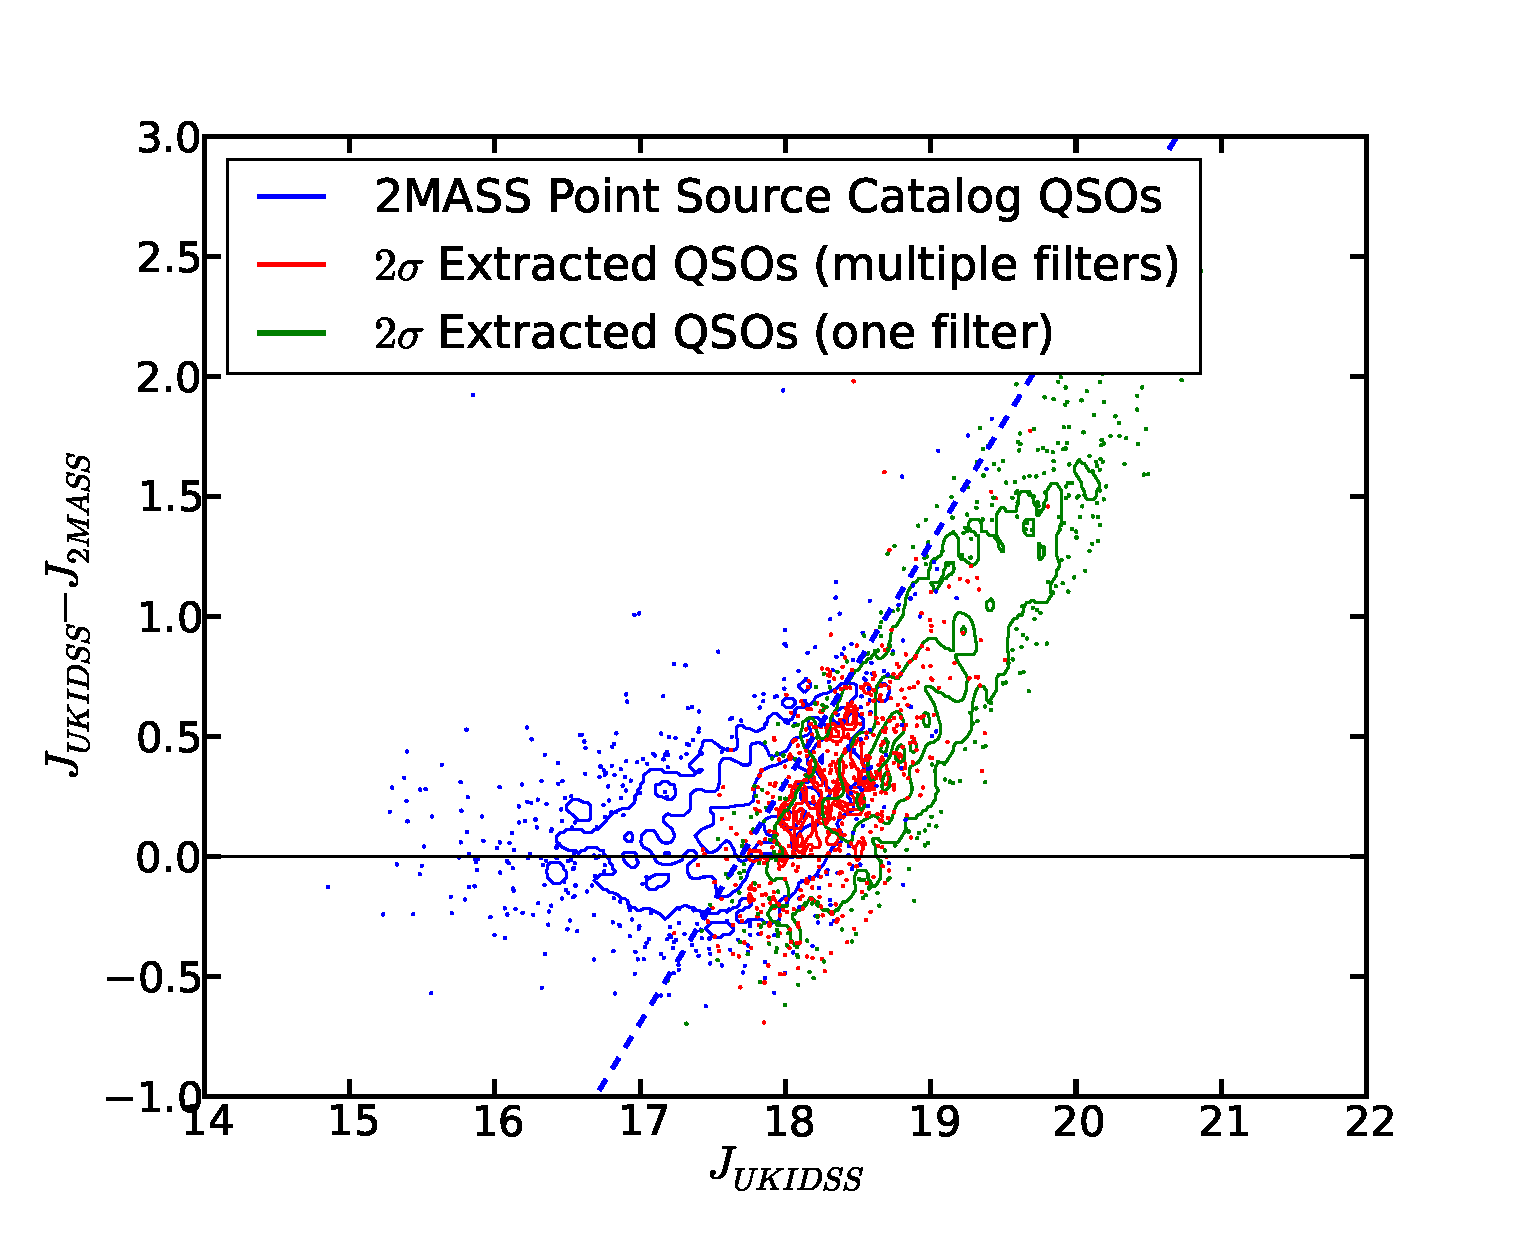
\includegraphics[width=3in]{images/Data/f3a} & 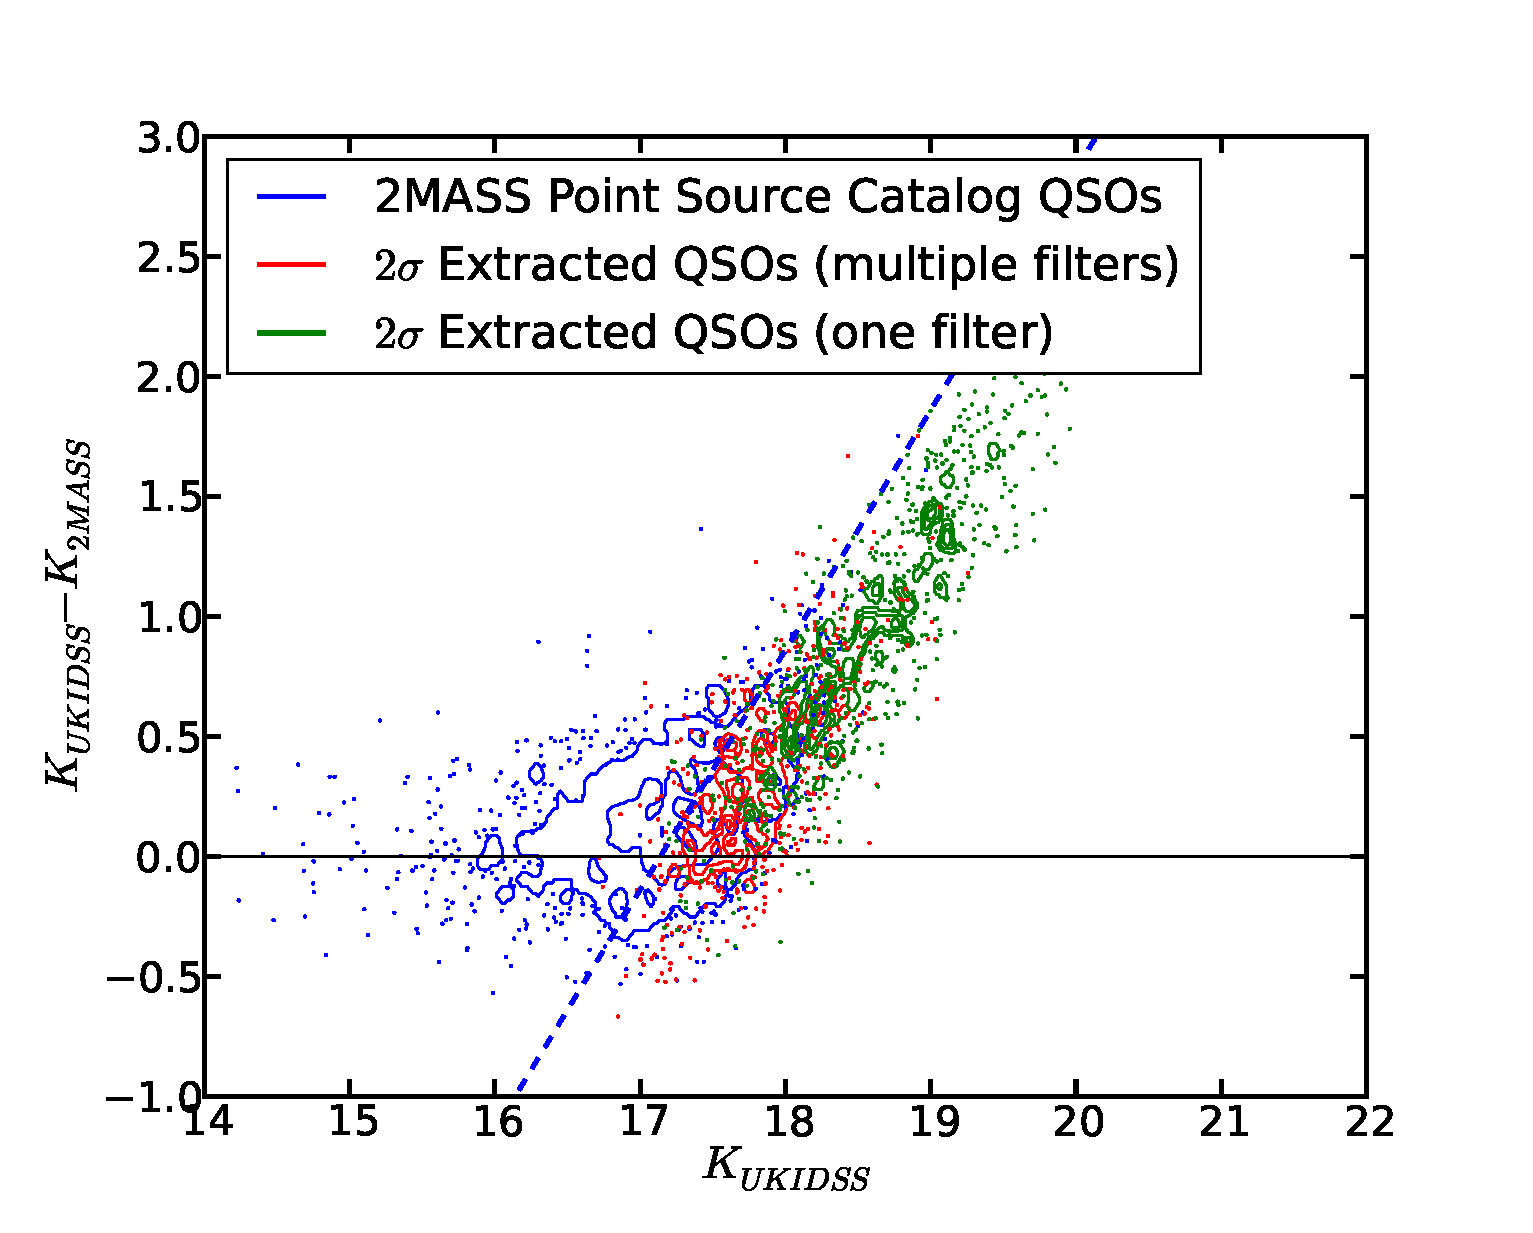
\includegraphics[width=3in]{images/Data/f3c}
 \end{tabular}
 
 \caption[2MASS vs. UKIDSS]{Contour-scatter plot showing the difference between the 2MASS and UKIDSS magnitudes vs. the UKIDSS magnitudes for the $J$ and $K$ filters. The blue contours/dots show the catalog 2MASS values, green shows the 2MASS $2\sigma$ extraction values with a detection in only one band, and red shows the rest of the extracted values. The blue dashed line shows the 2MASS point source catalog's limiting magnitude.
 The two surveys contain 12,130 quasars in common.  Green points were excluded as the errors are quite large (see text).  Similar results were found for the $H$ filter.}
 \label{2mass_v_ukidss}
\end{figure*}

\section{Mid-Infrared}

To extend our SEDs into the mid-IR, we included matches to the {\em WISE} final data release \citep{Wright:2010}.  The {\em WISE} bandpasses are generally referred to as $W1$ through $W4$ and have effective observed frame wavelengths of  3.36, 4.61, 11.82, and 22.13$\mu$m, respectively, for a typical quasar SED.  The matching was performed by taking all non-contaminated {\em WISE} point sources within $2''$ of an SDSS quasar as a match. This matching radius maximizes the number of true objects matched while also minimizing the number of false matches. Figure \ref{wise_sep} shows the number of {\em WISE} matches found as a function of separation distance from SDSS quasars. To ensure only the best matches were included, we also required that all matched quasars have S/N $\geq 10$ in both $W1$ and $W2$. In total, we have 85,358 matches to {\em WISE}; 
we estimate the false matching rate to be 1\% based on the number of matches obtained after shifting all {\em WISE} data by $200''$ in declination (red line in Figure \ref{wise_sep}). 
Since the {\em WISE} photometry was calibrated against blue stars it tends to overestimate the flux of red sources by about 10\% in the $W4$ band \citep{Wright:2010}, this correction has been applied to all quasars in our sample.

\begin{figure}[t]
 \centering
 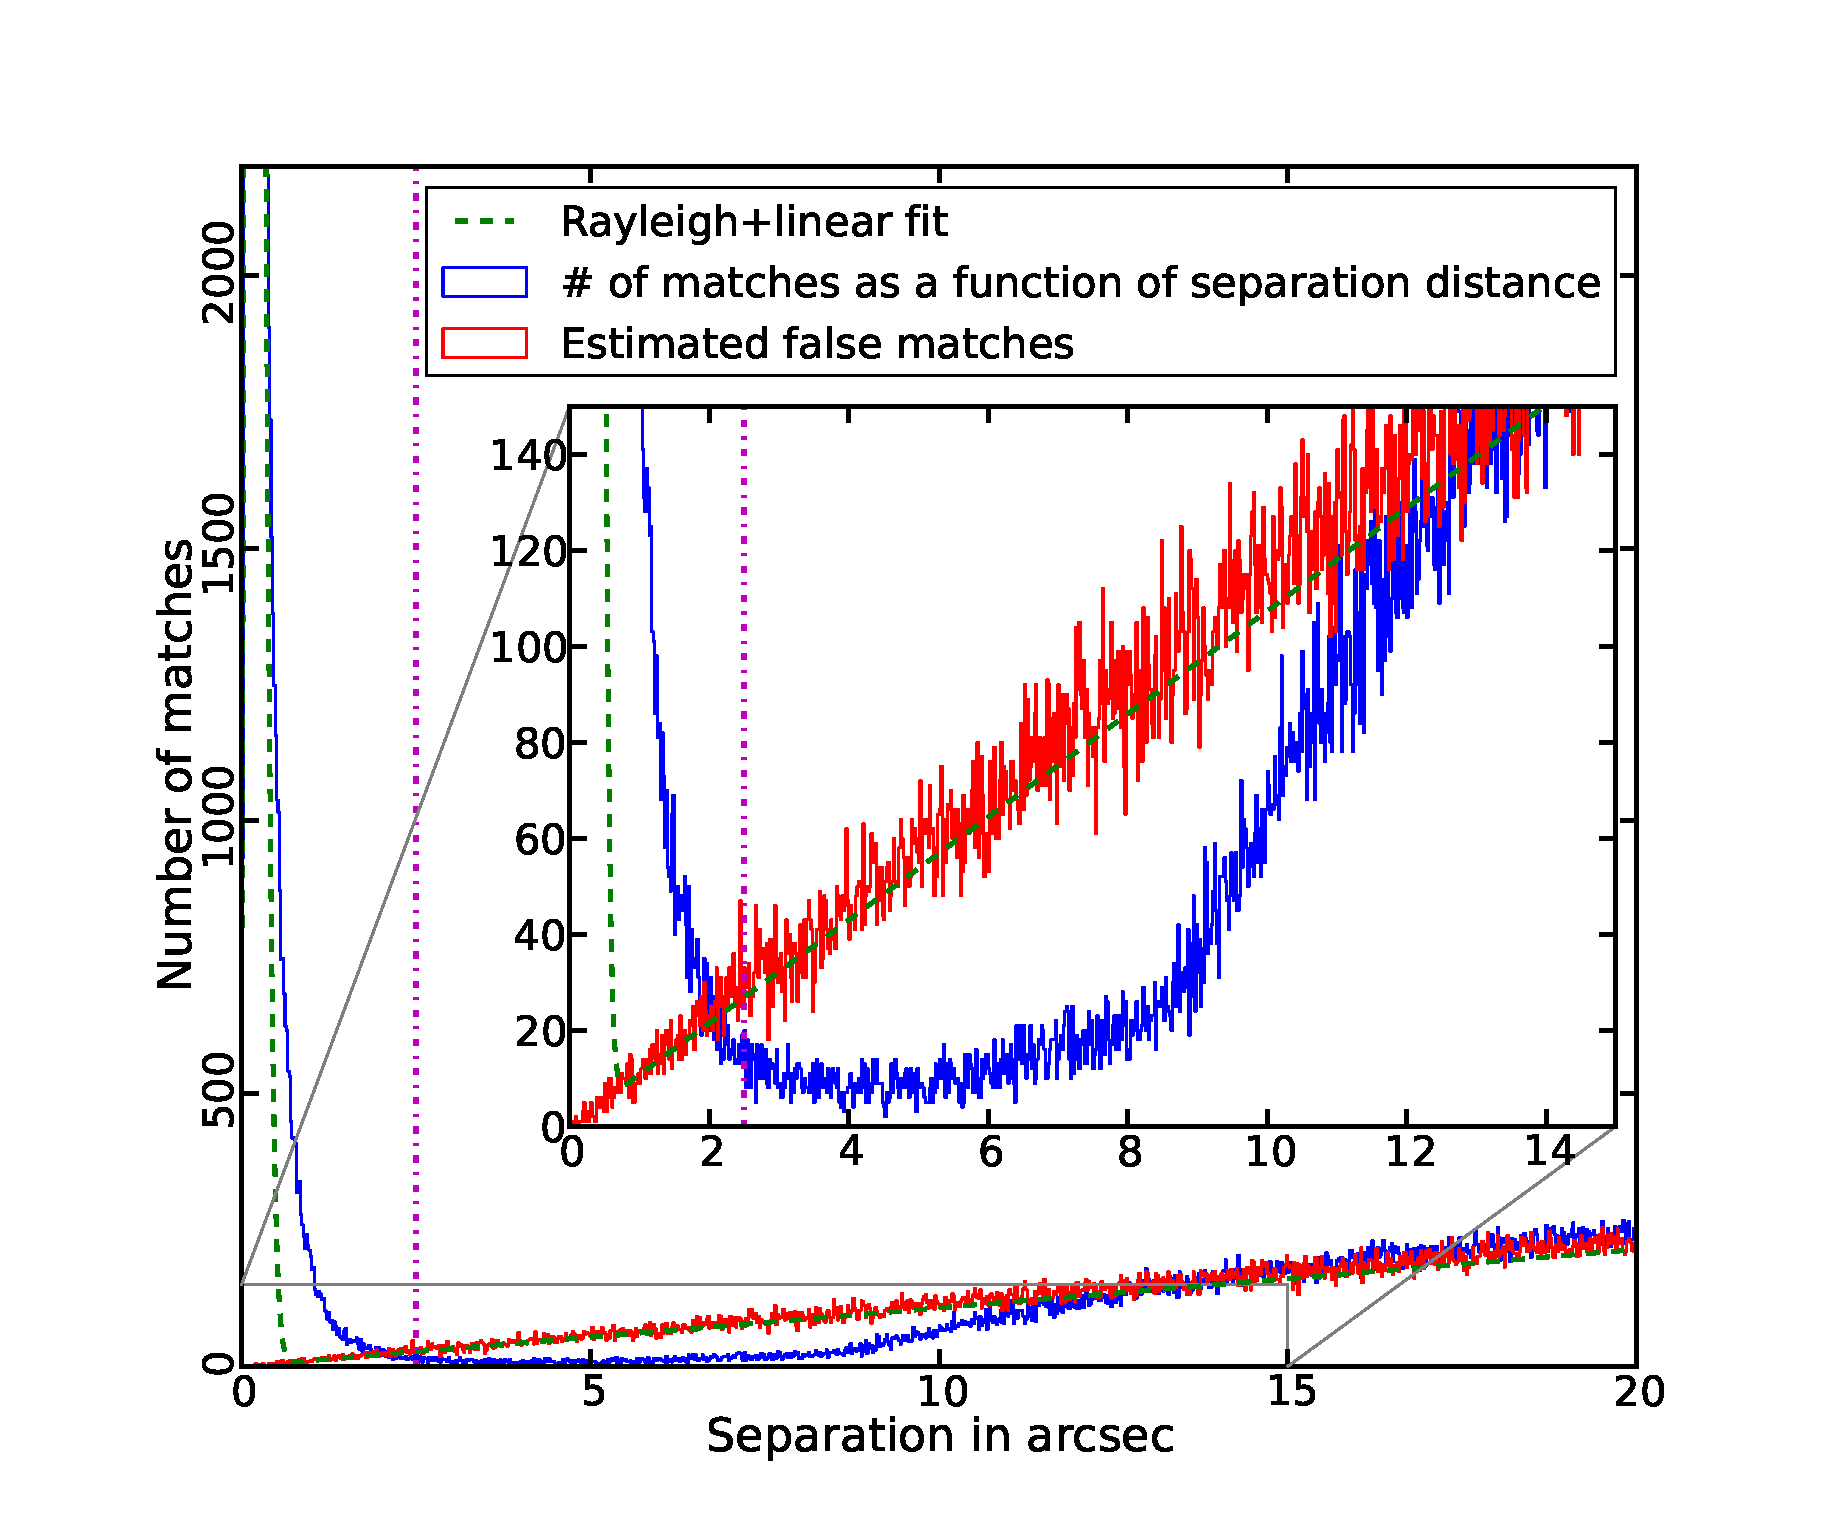
\includegraphics[width=5in]{images/Data/f4}
 \caption[{\em WISE} matching radius]{Angular separation between known quasars and nearby {\em WISE} sources (blue) and the known quasars with declinations shifted by 200$''$ (red).   The green curve shows the best fit expected distribution (Rayleigh distribution for small separations and linear growth for larger separations). The vertical magenta dot-dash line indicates the matching radius used.  As seen in the inset, the blue histogram does not follow the expected distribution; this is due, in part, to the large beam size of {\em WISE} (FWHM=$6''$).}
 \label{wise_sep}
\end{figure}

When available, {\em Spitzer} IRAC data were also included.  We specifically included data from the Extragalactic First Look Survey \citep[XFLS;][]{Lacy:2005}; Spitzer  Deep-Wide Field Survey \citep[SDWFS;][]{Ashby:2009}; SWIRE DR2 \citep{Lonsdale:2003}, including the ELAIS-N1, -N2, and Lockman Hole fields; S-COSMOS \citep{Sanders:2007}, and our own extraction of high redshift QSOs in stripe 82 (S82HIZ, program number 60139).  The fluxes for known SDSS quasars from the Stripe 82 program are reported here for the first time in Table \ref{data_table} ({\em Spitzer} source labeled as S82HIZ).  The IRAC bandpasses (ch1--ch4) have effective wavelengths of 3.52, 4.46, 5.67, and 7.7 $\mu$m for a typical quasar SED.  There are a total of 1196 matches to {\em Spitzer}.  For a small number of quasars ($\sim200$) both {\em Spitzer} and {\em WISE} data are available; in these cases, we use both data sets.  In Table \ref{data_table} all {\em Spitzer} and {\em WISE} fluxes are reported in AB magnitudes.

\section{Ultraviolet}

To extend the SEDs into the UV, we use {\em Galaxy Evolution Explorer} \citep[{\em GALEX}; ][]{Martin:2005} data when available.  The effective wavelengths for the near-UV (NUV) and the FUV bandpasses are 2267\AA\ and 1516\AA, respectively. Most of our matches are taken from \citet{Budavari:2009} who matched {\em GALEX}-GR6 to SDSS-DR7.  For this study, we have taken only the most secure matches; that is, only one SDSS quasar matched to only one {\em GALEX} point source.  This algorithm gives 14,302 matches and leaves out 53,782 quasars that have multiple SDSS sources matching to the same {\em GALEX} source.  In addition to these data, we include forced point-spread function (PSF) photometry \citep{Bovy:2011,Bovy:2012} on the {\em GALEX} images in the positions of the SDSS point sources, which adds 61,490 detections.  As with 2MASS, we only kept the extracted data with S/N $\geq 2$, and as with the \citet{Budavari:2009} matches, we limit the sample to those with no source confusion; this reduces the number of extracted quasars to 27,744.  Combining both sets, the total number of matches is 42,046.  All {\em GALEX} photometry has been corrected for Galactic extinction, assuming $A_{{\rm NUV}}= 8.741\times E(B-V)$ and $A_{{\rm FUV}}= 8.24\times E(B-V)-0.67\times E(B-V)^2$ \citep{Wyder:2007}.  The $E(B-V)$ values are taken from the \citet{Schneider:2010} catalog.  All the matched data are given in Table~\ref{data_table}.

\section{X-Ray} \label{X-ray}

To construct full SEDs, we must extend our data into the X-ray regime.  Due to comparatively limited sky coverage of sensitive X-ray observations, the number of our quasars with X-ray data is quite small compared to the size of the samples in the optical and IR.  For example, there are only 277 matches in the ChaMP data set \citep{Green:2009}.
So instead we take advantage of the careful work on mean X-ray properties as a function of UV luminosity as compiled by \citet{Steffen:2006}.  Specifically, we determine the X-ray flux of each quasar using the $L_{\rm UV}$--$L_{\rm X}$ relation that parameterizes the correlation between the 2500\AA\ and \twokev\ luminosity of quasars. We find the 2500\AA\ luminosity by extrapolation from the closest filter using an $\alpha_{\rm opt}=-0.44$ \citep{Vanden-Berk:2001}.  The \twokev\ luminosity is estimated using Equation \ref{just_eq} and our 2500\AA\ luminosities.  An X-ray energy spectral index $\alpha_x=-1$ (photon index $\Gamma=-2$) was assumed between \twohundredev\ and \tenkev\ \citep[e.g. ][]{George:2000}.  In this way, we can estimate the X-ray part of the SED for all of our sources rather than using just the small fraction of objects with robust X-ray detections. This process ignores the correlations between \aox\ (and \alphauv) and \ax\ as discussed in \citet{Kruczek:2011}; however, these trends are small as compared to the overall trend with luminosity.  

As a check we have compared our X-ray extrapolations to ChaMP data from \citet[][see Section \ref{sed}]{Green:2009}. In all cases we found the X-ray data to fall within the 1.5$\sigma$ limits of the \aox\ extrapolation. 

\section{The Dust Reddening Sample} \label{Dust_data}

For the analysis in Chapters~\ref{Dust} and~\ref{BH} we limit our sample to the uniformly selected point source quasars \citep{Richards:2006a}, leaving an initial sample of 55,772 quasars. This cut mitigates against any biases due to selection effects.

In order to better understand the dust present at a quasar's redshift, we further desire to minimize the effects of reddening caused by intervening galaxies.  We achieve this by removing 16,450 quasars that show signs of strong absorption line systems along the line of sight.
The presence of strong absorption lines in the spectrum of a quasar generally indicates that the light is passing through an intervening galaxy.  As dust in those galaxies can redden the quasar spectrum \citep{York:2006,Menard:2008,Khare:2012}, it is important to remove such quasars from our sample.
We specifically removed all quasars with at least two identified absorption lines (grade C or higher in the parlance of \citet{York:2005}) with a \ion{Mg}{2} line having an equivalent width (EW) $\geq0.3$\,\AA\ (York et al. 2014, in preparation).   These systems are thought to be associated with absorbing columns of $N_{\rm HI} \sim 10^{18-20} {\rm cm^{-2}}$ \citep{Churchill:2005,Prochaska:2010}.

This process yields a sample of quasars that is not selected preferentially because of radio properties and whose observed SED should be dominated by the physics of the accretion disk and dust reddening/extinction that is local to the quasar and/or the host galaxy.  As broad absorption line (BAL) quasars are seen to have different reddening properties \citep{Sprayberry:1992} and perhaps intrinsically different SEDs \citep{Weymann:1991,Reichard:2003b}, we split the sample into two groups: broad absorption line (BAL) quasars, as
identified by \citet{Shen:2011} and York et al. (2014, in preparation), and non-BAL quasars, containing 1,744 and 34,233 quasars respectively.

\begin{figure}[t]
\begin{center}
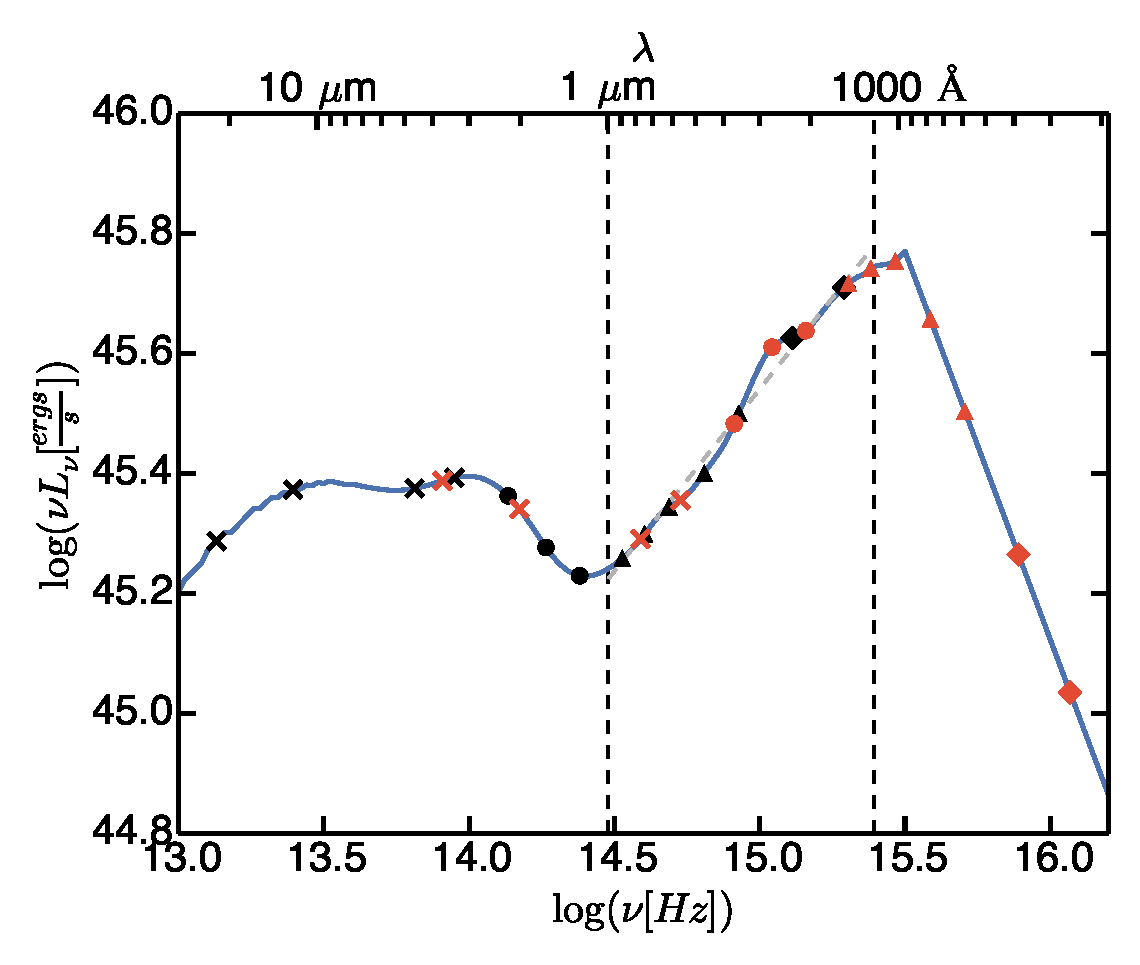
\includegraphics[width=5in]{images/Dust/f1}
\caption[Filter position vs. redshift]{\label{fig:sed_redshift} Position of various filters on the mean quasar SED (with the major spectral lines removed) for $z=0$ (black) and $z=5$ (orange).  The filters are from {\em WISE} (x's), 2MASS/UKIDSS (circles), SDSS (triangles), and {\em GALEX} (diamonds).  The vertical dashed lines show the range where the SED is well approximated as a powerlaw (dashed grey line $\alpha_\nu=-0.39$); all but the two reddest filters pass through this range for the redshift distribution of our sample.}
\end{center}
\end{figure}

For our dust analysis we only use the filters that fall between 1\,$\mu$m and 1216\,\AA\ in a quasar's rest frame (the portion consistent with a powerlaw). Because of these limits, only the following filters are used: {\em NUV} and {\em FUV} from {\em GALEX}, {\em ugriz} form SDSS, {\em JHK} from either 2MASS or UKIDSS, and {\em W1-2} from {\em WISE}.  Figure~\ref{fig:sed_redshift} shows the positions of these filters on the mean quasars SED (see Chapter~\ref{SEDs}) for $z=0$ (black) and $z=5$ (orange).  This mean SED has a powerlaw index of $\alpha_\nu=-1.39$ (grey dashed line) and the small blue bump is visible at $\sim3500$\,\AA.

\section{Black Hole Masses} \label{BH_data}

\begin{figure}[t]
\begin{center}
 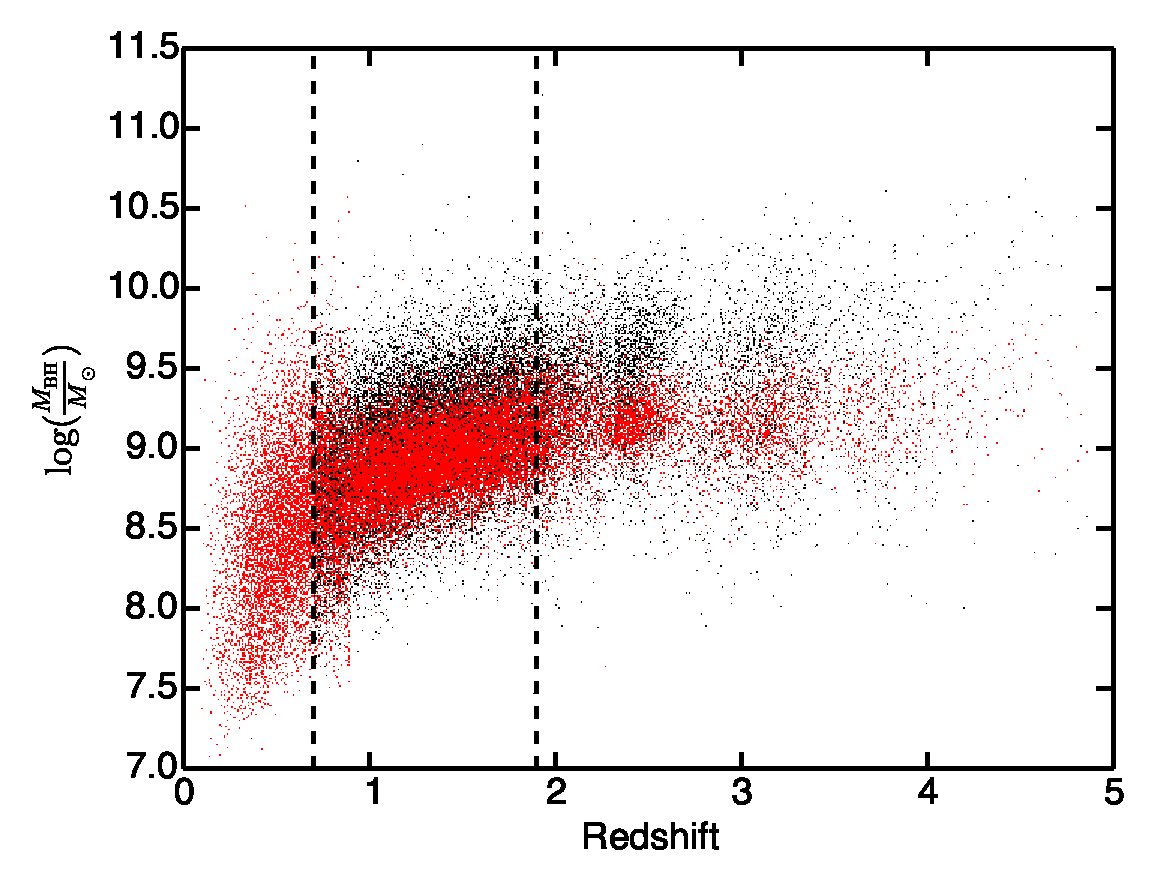
\includegraphics[width=5in]{images/BH/f1}
 \caption[$\mbh$ vs. Redshift]{\label{fig:shen_update}$\mbh$ vs. redshift for the \citet{Shen:2011} masses (black) and the re-calibrated masses used in this work (red). The vertical dashed lines indicate the redshift for transitioning between the different spectral line relations (H$\beta$, \ion{Mg}{2}, and \civ\ from left to right).}
\end{center}
\end{figure}

To build a catalog of $\mbh$ for our sample we began with the masses presented in \citet{Shen:2011} and matched them to the non-BAL quasar sample from \S\ref{Dust_data}.  These masses are estimated using the width of H$\beta$ ($z<0.7$), \ion{Mg}{2} ($0.7\leq z <1.9$), or \civ\ ($z\geq1.9$) using the $R_{\rm BLR}$--luminosity relations from \citet[][H$\beta$ and \ion{Mg}{2}\footnote{The \ion{Mg}{2} relation was updated in \citet{Shen:2011}}]{McLure:2004}, \citet[][H$\beta$ and \civ]{Vestergaard:2006}, and \citet[][\ion{Mg}{2}]{Vestergaard:2009}.  In the language of Equation~\ref{eqn:r_l} these relations are:

\begin{center}
\begin{tabular}{rl}
 %$(a,b) = (0.672, 0.61)$, & MD04; H$\beta$ \\
 $(a,b) = (0.910, 0.50)$, & VP06; H$\beta$ \\
 $(a,b) = (0.740, 0.62)$, & S11; \ion{Mg}{2} \\
 $(a,b) = (0.660, 0.53)$, & VP06; \civ \\
 %$(a,b) = (0.860, 0.50)$, & VO09; \ion{Mg}{2}
\end{tabular}
\end{center}

All of the masses in the \citet{Shen:2011} catalog assume $\Delta V^2 \propto {\rm FWHM}^2$, an assumption that has been shown to introduce significant scatter when compared to RM masses \citep{Wang:2009,Rafiee:2011,Peterson:2011,Denney:2012,Denney:2013,Park:2013}.  As a result, we use the updated scaling relations (using Equation~\ref{eqn:r_l_gamma}) for \ion{Mg}{2} and \civ\ as presented in \citet{Rafiee:2011} and \citet{Park:2013}:
\begin{center}
\begin{tabular}{rl}
 $(a,b,\gamma) = (7.25, 0.51, 1.27)$, & RH11; \ion{Mg}{2}  \\
 $(a,b,\gamma) = (7.48, 0.52, 0.56)$, & P13; \civ \\
\end{tabular}
\end{center}
Additionally, we included the intrinsic scatter for each of these relations into the uncertainty estimates for each mass.
Figure~\ref{fig:shen_update} shows $\mbh$ as a function of redshift for the \citet{Shen:2011} masses (black) and the re-calibrated masses used in this work (red). The re-calibrated masses are systematically smaller than the original catalog masses.

For these updated black hole masses we have not taken into account the effects of extinction within the quasar itself (see Chapter~\ref{Dust} for more details).  This correction turns out to be small and on average increases $\mbh$ by 0.02 dex, and in most cases (99\% of the sample) the ``de-reddened'' masses are within $1\sigma$ of the ``reddened'' masses.  Given how small this correction is we do not apply it to our sample.

Recent work \citep{Denney:2012,Denney:2013,Kratzer:2014} has cast doubt over estimating $\mbh$ based on the \civ\ line using the survey quality spectra from SDSS.  In particular \citet{Denney:2013} argue that the low $S/N$ of the SDSS spectra do not allow for the proper characterization of the \civ\ line (e.g. line dispersion) leading to higher scatter (and higher uncertainties) when compared to the more reliable H$\beta$ masses.  Although these issues are present within our data, we still include the \civ\ masses in the data analysis of Chapter~\ref{BH}.  However, our analysis weights each mass by its uncertainty, so even when we removed the \civ\ masses from our sample the results of our analysis do not change.  
% general trends found in our data.  